\documentclass[a4paper,conference]{IEEEtran}
\usepackage{cite}
\ifCLASSINFOpdf
  % \usepackage[pdftex]{graphicx}
  % declare the path(s) where your graphic files are
  % \graphicspath{{../pdf/}{../jpeg/}}
  % and their extensions so you won't have to specify these with
  % every instance of \includegraphics
  % \DeclareGraphicsExtensions{.pdf,.jpeg,.png}
\else
  % or other class option (dvipsone, dvipdf, if not using dvips). graphicx
  % will default to the driver specified in the system graphics.cfg if no
  % driver is specified.
   \usepackage[dvips]{graphicx}
  % declare the path(s) where your graphic files are
   \graphicspath{{./pics/}}
  % and their extensions so you won't have to specify these with
  % every instance of \includegraphics
   \DeclareGraphicsExtensions{.eps}
\fi
\hyphenation{op-tical net-works semi-conduc-tor}

\begin{document}
%
% paper title
% can use linebreaks \\ within to get better formatting as desired
\title{Pragmatics Dependent Hardware Design}


% author names and affiliations
% use a multiple column layout for up to three different
% affiliationsy
\author{\IEEEauthorblockN{
Taras Zakharchenko \IEEEmembership{Student Member, IEEE}
}
\IEEEauthorblockA{National technical university of Ukraine\\
``Kyiv polytechnic institute''\\
Ukraine, Kyiv\\
Email: taras@ieee.org}}

% make the title area
\maketitle


\begin{abstract}
%\boldmath
In the paper described a new hardware design metodology, in which pragmatics of design goal has the most significant influence on design ever. The author showed  basics of pragmatics dependent approach and proposes solution for automated transition from semantic notation of solution of problem given to specific syntaxes, described its implementation.
\end{abstract}

\begin{keywords}
reconfigurable hardware, adaptive computing, compositional design.
\end{keywords}
% no keywords

\IEEEpeerreviewmaketitle

%The Introduction serves to help the reader understand our
%three key questions: Why is this a new and important problem?
%What has been done before? How does your research bring
%significant new understanding to the field? The reader should
%find enough information to understand why your research was
%necessary, without having to refer to other source material or
%published works [7]. The introduction should be concise, no
%more than one or two pages. It is written in the present tense.
%Your introductory paragraph should start with what is generally
%known about your subject. Then move step by step through
%more detailed information, ending with a description of the
%specific problem or hypothesis your article will discuss. Try to
%use an attention-grabbing statement to hook the reader [10]
%while being careful not to sensationalize your results.
%In the next few paragraphs, refer to the published research to
%show what is already known about your subject and why your
%work is needed. Do not try to include everything from your
%literature review. Your goal is to orient the reader to the most
%relevant studies. Explain how each earlier study relates to your
%own approach to the problem. Does it have limitations? Does it
%make different assumptions [11]? Show your readers how your
%study builds upon or is different from this existing work. If you
%have published an earlier version of your work, for example as a
%conference or journal article, you must explain how the current
%study builds upon your own prior work [3].
%After you have explained the historical context of your work,
%introduce your hypothesis and provide a general description of
%the results you have obtained. You will flesh these out more
%fully later in the article, but providing an overview here motivates
%your audience to read on. At the end of your introduction, tell
%the reader how the article is organized. This will allow readers to
%move to sections of particular interest, if they wish.

%Why is this a new and important problem?
%What has been done before? 
%How does your research bring significant new understanding to the field? 
\section{Introduction}
Pragmatics dependent hardware depends solely on goals required to achieve with its development, the pargmatics. Noramally, hardware and software development processes depend on many other factors. For example, we want to develop one complicated computing solution. There are few options: to write new software with existant programming language for specific processor or to develop own hardware accelerator for this purpose and run it on reconfigurable platform along with other pieces of similar hardware. Thinking about new programming language design, designer unable to forsee all possible applications and design unvidersal programming language. Thinking about new CPU design, designer unable to predict all kinds of its usage, one relies only on general case, restricting software engineer's freedom of mind, who will use programming languages and CPU afterwards. This problem especially important nowadays, when chip designers will be unable to maintain Moore's low soon \cite{mooremaxwell} limited by fundamental laws.

There are a plenty ways to deal with the problem and plenty efforts toward solution undertaken. A classification of reconfigurable patterns was developed by DeHon et al. \cite{reconfigurable_patterns} It is step forward to optimal hardware generation. Another effort toward multiplatform code was undertaken by M. Tarver, creator of LISP based Shen language, which produces program code in various other languages \cite{tarver2013book}. It can be modified to produce HDL too. Thus, margin between hardware and software will be removed.

The design process needs a systematic approach. Consider computing device as a system, this system may be treated as one maximum closed. Output of the system depends only on input data and obfscure internal state.\\
Counterexample is a hardware description language (HDL). It is maximum opened system. The closed part in this case is only set of basic operations and control structures.

It is important to find a tradeof between opened and closed design systems before start design process depending on pragmatics of the given problem. As result, open-closed system will be optained, which will produce device designs.\\
The other feature of proposed soultion is consideartion of a problem in different aspects: pragmatic, semantic, syntactic. Pragmatic aspect reflects intents of one who set the problem, a matter of it. Semantic aspect is actual solution of the problem, formed only by solution designer it does not depend on any specific tachnical aspects. It is formal expression of the idea. Syntactic aspect is implementation of semantic of solution of the problem for specific platform. All these aspects are separable one from another. In programming languages, there is no such separation. Semantic of problem solution id dissolved in programming language syntax. We propose to separate them explicitly. This will help to save investments in solution development, because such approach will make the solution portable to other platforms, HDL, programming languages. Pragmatic produces semantic, sematic produces syntax.

In this paper attention mostly payed to automated transistion from semantic to syntax. I provided examples for HDL and assembly language in order to prove that semantic indeed does not depend on syntax even in such fundamentally different cases. The purpose of the research is to automate syntax production and provide handy development environment for developer.

\section{System Architecture}
First, lets get familiar with mathematical fundamentals of proposed solution. They were proposed by A. Maltsev (???)\cite{}. The point is that every program is function. The function maps input to output, one memory region to another. Next statement that function may be decomposed on simplier parts, compositions of basic operations, to be computable by specific computer. Together with carrier set (datatype, which processed), the set of operations and compositions forms algebraic structure. This algebraic structure formed depending on pragmatics of problem given. Here compositions are operations over set of operations and other compositions. Due to usage of algebraic structures, we are able to design mathematically correct hardware and programms. Because they designed on correct basis. Now consider programming language, it is based on a limited set opeartions, which were proposed by programming language developers, who, in the most cases, did not substantiated the selection.\\
Lets have a closer look at design process in action. First, designer considers pragmatic aspect of the given problem and selects the most adquate set of operations and compositions, substantiating it. For example, there is a problem to compute solution of quadratic equation ($a \cdot x^2 + b \cdot x + c = 0$). Having many aspects of the problem analyzed, the designer chooses simple arithmetics as set of basic operations and application with primitive recursion as compositions.\\
The next step is to write down semantics of the solution. For today only man can produce semantics, it is complicated and too creative work for machine. It may only assist designer on this step. So the solution is written as the designer understands it.
$\\
D = \sqrt{b^{2} - 4 \cdot a \cdot c}\\
x_{1} = \frac{-b + D}{2 \cdot a}\\ 
x_{2} = \frac{-b - D}{2 \cdot a}\\
$
But the set of opeartions here is different to one that chosen. So the solution must be rewritten in the chosen set of operations and compositions. Square root and squaring operations are not in the set of chosen opertions. If they was perviously implemented on selected algebraic structure, the next step begins. If not, the designer implements square root for the algebraic structure. For example, square root operation is not implemented. A decision to use Heron's method  was made ($ x_{n+1} = \frac{1}{2}(x_{n} + \frac{a}{x_{n}}) $). For a reasonable count of steps and adequate result will be achieved. Now that operations in Heron's formula computer understands.\\
Now user can automatically produce syntax of the solution for specific platform. The system teakes as input semantic representation of the solution, then resolves unresolved operations and compositions. After resolving, it converts the solution to a platform specific syntax. In which the algebraic structure was implemented, for example, HDL. Later this algebric structure may be supplemented with other operations and compositions.\\


\section{Implementation}
I have successfully implemented software for transition from semantic representation to syntax as a proof of concept. I have chosen Church's algebra as algebraic structure the system. Basic operation of the algebra are: increment, assignment to zero, selection argument by specific index. Compositions are: application, primitive recursion, minimization.

On the input semantics solution is passed. The software parses semantic representation of solution into semantic tree according to rules choosen for semantics formalization. Leaves of the tree are input variables and constants and non-terminal vertices are compositions and metacompositions (compositions of compositions and operations).

It is selected JSON representation of the tree. Every vertex represented in fllowing form:\\
\texttt{
\{\\
\indent "name":character string,\\
\indent "id":numeric identifier,\\
\indent "static":[parameter list],\\
\indent "arguments":[{"no":1, "value":argument value},...]\\
\}\\
}

The \texttt{name} field is mnemonic designator of function, performed by specific vertex, \texttt{id} field is numeric vertex identifier for non-ambigous interpretation of vertices. \texttt{static} field is list of vertex parameters. They can be terms and/or values. Here term means semantic representation of other tree. Term may be an argument of compositions which are to manipulate them. The \texttt{arguments} field is a list of function(non-terminal vertex) arguments, in other words, list of vertices, which are connected to this one. Every element of list characterized by number \texttt{no} and value \texttt{value} which is vertex. A tree, which represents expression \texttt{add(IN0, mul(IN1, IN2))} looks like this:\\
\texttt{
\{\\
\indent "arguments": [\\
\indent \indent \{\\
\indent \indent \indent "value": "IN0",\\
\indent \indent \indent "no": 0\\
\indent \indent \},\\
\indent \indent \{\\
\indent \indent \indent "value": \{\\
\indent \indent \indent \indent "arguments": [\\
\indent \indent \indent \indent \indent \{\\
\indent \indent \indent \indent \indent \indent "value": "IN1",\\
\indent \indent \indent \indent \indent \indent "no": 0\\
\indent \indent \indent \indent \indent \},\\
\indent \indent \indent \indent \indent \{\\
\indent \indent \indent \indent \indent \indent "value": "IN2",\\
\indent \indent \indent \indent \indent \indent "no": 1\\
\indent \indent \indent \indent \indent \}\\
\indent \indent \indent \indent ],\\
\indent \indent \indent \indent "static": [],\\
\indent \indent \indent \indent "name": "mul",\\
\indent \indent \indent \indent "id": "384009"\\
\indent \indent \indent \},\\
\indent \indent \indent "no": 1\\
\indent \indent \}\\
\indent ],\\
\indent "static": [],\\
\indent "name": "add",\\
\indent "id": "415422"\\
\}
}

\begin{figure}
\centering
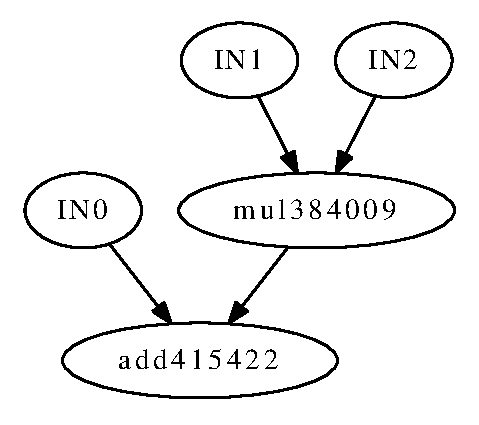
\includegraphics[width=2in]{source}
\caption{Graph representation of \texttt{add(IN0, mul(IN1,IN2))}}
\label{source_graph}
\end{figure}

\begin{figure*}
\centering
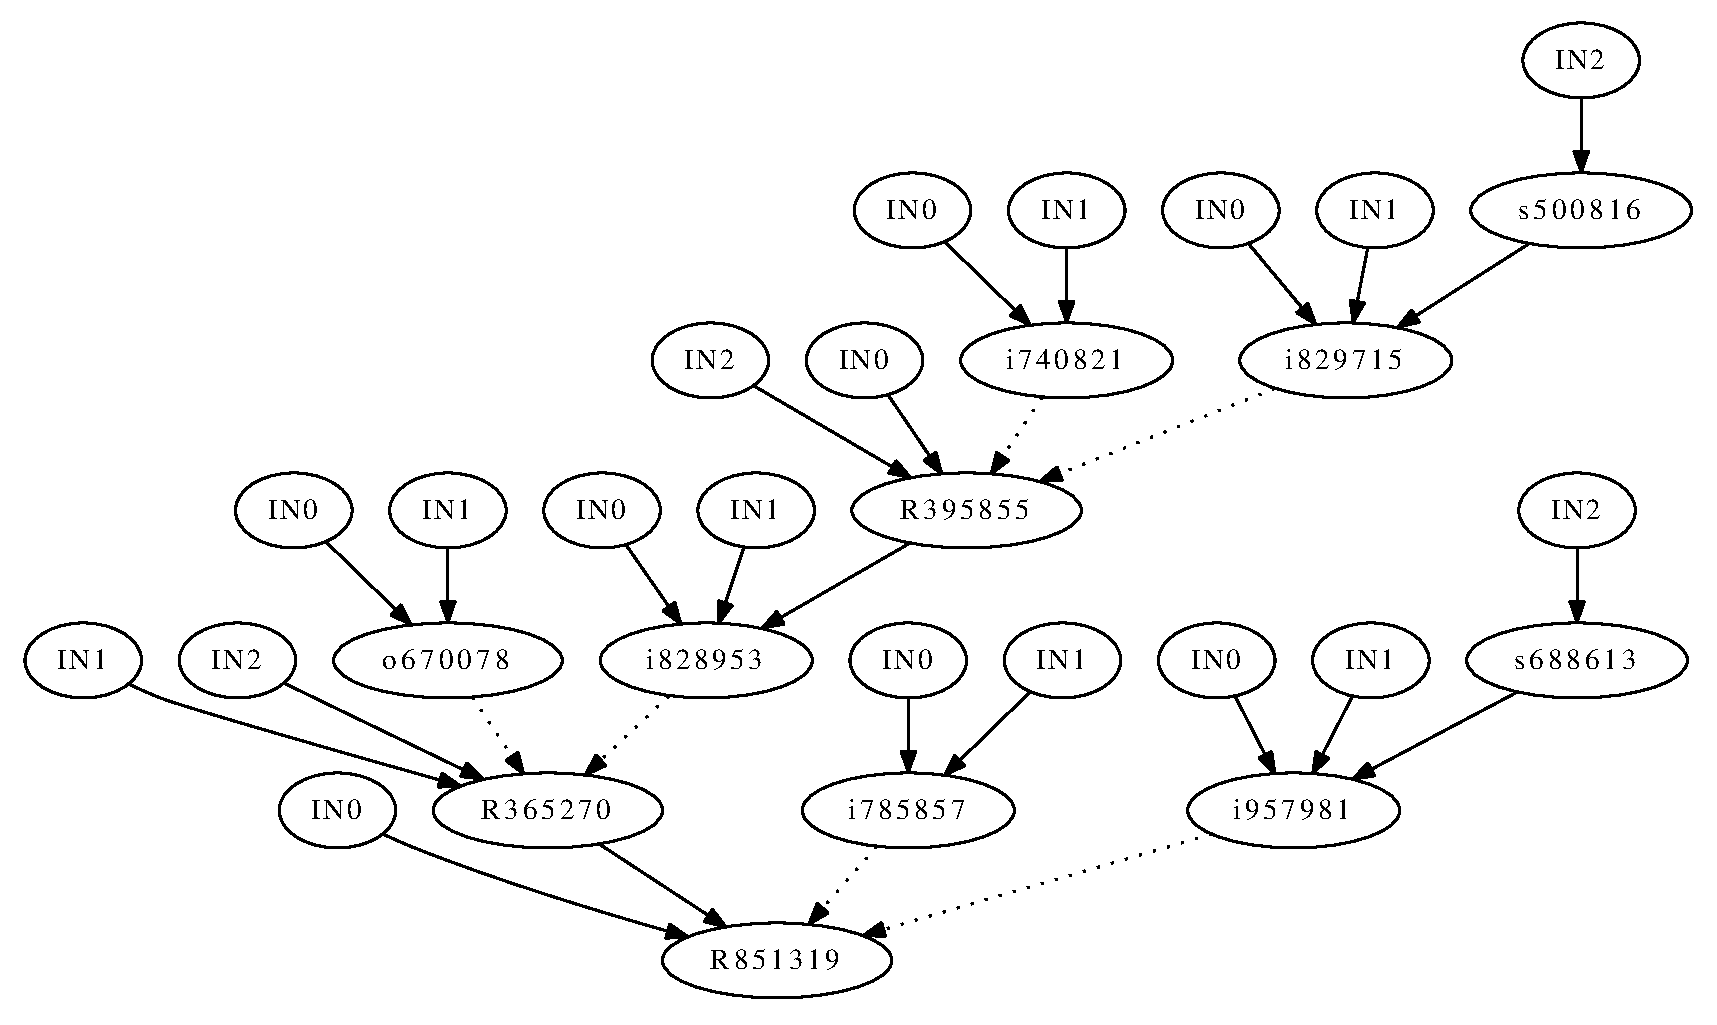
\includegraphics[width=5in]{primitive}
\caption{Graph representation of \texttt{add(IN0, mul(IN1,IN2))} after substitution.}
\label{primitive_graph}
\end{figure*}

For convenience the system produces tree representation of expression  (fig. ~\ref{source_graph}). It has some non-terminal vertices computer not familiar with, but algorithm of the system can replace them substituting instead non-familiar non-terminal vertices compositions of familiar ones(fig. ~\ref{primitive_graph}). Such compositions represented in JSON format too. For example operation of addition in terms of Church algebra:\\
\texttt{
\{\\
\indent name:R,\\
\indent id:\%ID1\%,\\
\indent static:[\\
\indent \{\\
\indent \indent name:i,\\
\indent \indent id:\%ID2\%,\\
\indent \indent static:[0],\\
\indent \indent arguments:[\\
\indent \indent \indent \{no:0, value:IN0\},\\
\indent \indent \indent \{no:1, value:IN1\}\\
\indent \indent ]\\
\indent \},\\
\indent \{\\
\indent \indent name:i,\\
\indent \indent id:\%ID3\%,\\
\indent \indent static:[2],\\
\indent \indent arguments:[\\
\indent \indent \indent \{no:0, value:IN0\},\\
\indent \indent \indent \{no:1, value:IN1\},\\
\indent \indent \indent \{no:2, value:\{\\
\indent \indent \indent \indent name:s,\\
\indent \indent \indent \indent id:\%ID4\%,\\
\indent \indent \indent \indent static:[],\\
\indent \indent \indent \indent arguments:[\\
\indent \indent \indent \indent \indent \{no:0, value:IN2\}\\
\indent \indent \indent \indent ]\\
\indent \indent \indent \indent \}\\
\indent \indent \indent \}\\
\indent \indent ]\\
\indent \}\\
\indent ],\\
\indent arguments:[\\
\indent \indent \{no:0, value:\%IN0\%\},\\
\indent \indent \{no:1, value:\%IN1\%\}\\
\indent ] \\
\}\\
}

Dotted lines on the figure~\ref{primitive_graph} denote that child vertex is a static parameter. Vertices with names starting with "o" are zero generators. Vertices with names starting with "s" perform operation of increment. Vrtices with name starting with "i" perform operation of selection one of arguments to send it to output, using static parameter, which denotes index of selected argument. Vertices with names starting with "R" represent primitive recursion composition. Terminal vertexes with names starting with "IN" represent arguments of the function in case when when a path from root to terminal vertex constists only of solid lines, in other case these are local inputs of compostion's static parameters.

The system produces HDL representation from such tree. To prove universality of the system, Moreover, generation of x86\_64 assembly was added as well. The system developed with Python programming language. It is agile enough to modify the system quickly.

\section{Conclusion}
The described approach has a long history, but means to implement it and need in it emerged only nowadays. The state of microelectronic industry requires reconfigurable logic as one of the possible ways to avoid crysis which may come with the end of the Moore's low. A software proposed in the paper to compile sematic representation of problem's solution to syntax representation plays an important role in the approach, as one of the parts of it, which could be fully automated. That is why during the research a concept of the adaptive development environment was developed at first time. The software is a proof of concept rather the one which ready for use in the industry, but it demonstrates ability to remove margin between software and hardware compiling the same semantic description of problem's solution into x86 assembly snd Verilog code. It is expected that the approach will produce more reliable hardware and software, and will increase portability.
\bibliographystyle{IEEEtran}
\bibliography{pragmatic_dependent}{}


\end{document}


